\subsection{Data Cleaning and Preprocessing}

The overall workflow that we followed throughout this study can be found in Figure~\ref{fig:journey-roadmap}. Our data preprocessing strategy explicitly addresses the challenge of working with large-scale thermal comfort databases that contain inevitable data quality issues while preserving the statistical power of the combined dataset.

\begin{figure}
    \centering
    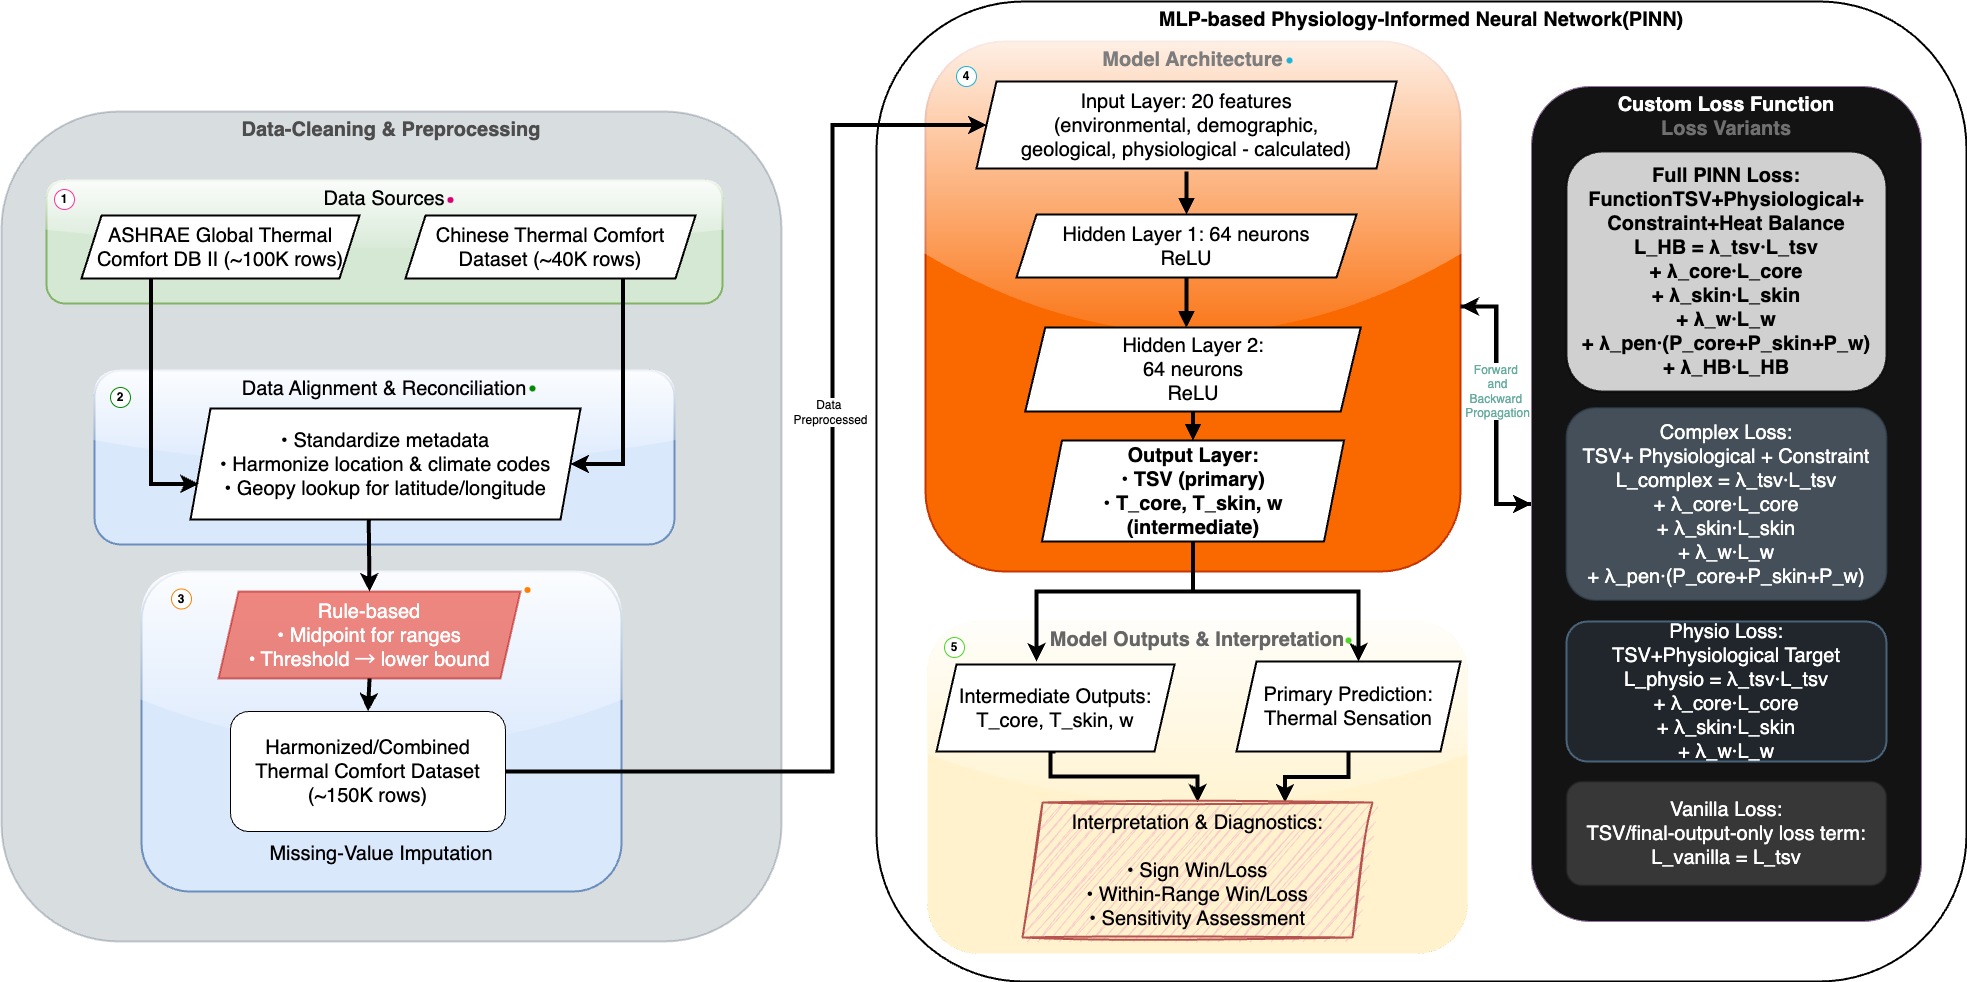
\includegraphics[width=0.95\linewidth]{figures/PINN_noVAE.png}
    % \caption{Overall workflow of our Physiology-Informed Neural Network Investigation}
    \caption{Overall workflow of our Physiology-Informed Neural Network Investigation. (Note: Figure will be updated with larger text sizes for final submission.)}
    \label{fig:journey-roadmap}
\end{figure}

\paragraph{Dataset Harmonization and Quality Assessment} As illustrated in this overview, we initiated our pipeline with two distinct datasets: one from ASHRAE (103,435 entries) and another from China (41,726 entries). The ASHRAE database II originally comprised environmental measurements paired with its native metadata. However, an initial mapping challenge necessitated the standardization of this metadata. Specifically, we remapped location-specific attributes—such as city names, climate zones, and building types—to a consistent schema, thereby ensuring that each ASHRAE record was enriched with accurate geographic information. Geospatial tool packages like \texttt{geopy} were employed to verify and, when necessary, supplement the latitude and longitude data, ensuring reliable spatial identification. 

Initial analysis revealed significant data completeness disparities: while environmental variables like air temperature were well-represented ($>$95\% completeness), demographic variables showed substantial missing data (age: 78\% complete, gender: 82\% complete, height: 65\% complete, weight: 63\% complete). After harmonizing the ASHRAE database II, it was concatenated with the China dataset, which had its own complementary set of measurements and metadata. This concatenation was carefully performed by aligning records along common temporal and spatial dimensions, thereby forming a unified dataset that integrated environmental conditions and subject-related information from both sources.

\paragraph{Physics-Informed Imputation Strategy} Subsequent cleaning steps addressed data inconsistencies and missing values across the unified dataset. Rather than discarding incomplete records—which would have eliminated approximately 45\% of the combined dataset and introduced sampling bias toward studies with complete demographic collection—we implemented a physics-informed imputation strategy. Missing demographic and environmental variables, specifically age, gender, height, and weight—were imputed using defaults derived from established domain-specific standards (e.g., those recommended by Gagge). This approach ensures that imputed values remain within the operational ranges of the Gagge and JOS-3 physiological models, preventing extrapolation errors in subsequent physiological variable generation.

In the case of age, where entries included both precise numeric values and ranges, our approach was to compute a representative numerical value: ranges were replaced by their midpoint, and when expressed as a threshold (e.g., "$>60$"), the lower bound was retained. Critically, our PINN framework's physics constraints provide built-in validation for this imputation strategy. Because the neural network must satisfy energy balance equations and physiological range constraints regardless of input demographics, imputation errors that would lead to physiologically implausible combinations are automatically corrected during training.

We also performed another step upon the 49 features to create joined categorical features based off our understanding by creating additional joined categorical features such as \textit{country-season}, \textit{climate-country}, etc. Additionally, categorical variables were uniformly converted to numerical codes using label encoding to facilitate downstream deep learning applications. 

\paragraph{Validation of Internal Consistency} These preprocessing measures ensured that the final dataset was both internally consistent and robust against missing or non-standardized inputs, which is especially critical for PINNs due to its sensitivity to input data quality. Our approach provides multiple validation layers: (1) cross-checking environmental variables for physical plausibility, (2) verifying clothing insulation values against seasonal and climate data, and (3) most importantly, requiring that physiological variables generated from imputed demographics satisfy energy balance constraints during model training, providing continuous validation of internal consistency at the physiological level. The final harmonized dataset contained 145,161 entries with 20 selected features after removing variables with less than 50\% data availability.

\subsection{Physiological Variables Generation}

Physiological parameters, critical for our analysis, were not directly measured in the initial datasets; rather, they were derived computationally from the available environmental and subject data. This computational approach directly addresses a fundamental challenge in thermal comfort research: how to obtain reliable physiological estimates when direct measurements are unavailable, while ensuring the resulting data remains physiologically plausible for machine learning applications.

\paragraph{Rationale for Dual-Model Approach} We employed both Gagge's two-node model and the JOS-3 model to create a robust ensemble of physiological estimates that mitigates individual model limitations. Gagge's model provides well-validated steady-state estimates with established relationships to thermal sensation, while JOS-3 offers more detailed segmental modeling that captures individual demographic variations. Rather than viewing this as a limitation, our PINN framework leverages this dual approach as a strength: by training on estimates from both models and enforcing physics constraints, the network learns to extract consistent physiological patterns while being robust to model-specific artifacts.

\paragraph{Gagge Model Implementation and Validation} We utilized the \texttt{pythermalcomfort} library to implement Gagge's two-node function, computing key physiological outputs—such as $T_{core}$, $T_{skin}$, sensible heat flux, and additional thermal indices—based on inputs including air temperature, mean radiant temperature, air velocity, relative humidity, clothing insulation, and metabolic rate. While concerns about JOS-3's validation on nude subjects are noted, Gagge's model was specifically developed and validated for clothed occupants in building environments, making it highly appropriate for our application. The model's clothing area factor ($f_{cl}$) calculations are based on established relationships with clothing insulation values that are directly available in our datasets.

\paragraph{JOS-3 Model Integration and Uncertainty Management} In parallel, we used the JOS-3 model to simulate further aspects of human thermoregulation. The JOS-3 model integrated individual-specific parameters—namely, height, weight, age, and gender—to generate additional physiological estimates, including simulated $T_{core}$, $T_{skin}$, basal metabolic rate, and thermogenic responses. While JOS-3 requires local clothing parameters that are often unavailable in thermal comfort databases, our physics-informed approach addresses this limitation through constraint-based regularization. When local clothing insulation values ($f_{cl}$) are missing, the model uses established correlations with overall thermal insulation, and any resulting uncertainties are mitigated by the energy balance constraints in our PINN framework.

\paragraph{Model Fusion and Physics-Based Validation} The outputs from the JOS-3 simulation were merged with those obtained from the Gagge's two-node function through a systematic approach that leverages the strengths of both models. Rather than simple averaging, we treat each model's outputs as independent estimates and allow our PINN's physics constraints to determine the optimal weighting during training. This fusion approach is validated through the energy balance constraint: $Q_{balance} = (M - W) - (Q_{conv} + Q_{rad} + Q_{evap} + Q_{res}) \approx 0$, which ensures that the final physiological estimates from either model must satisfy fundamental thermodynamic principles.

\paragraph{Addressing Reconstruction Validity Concerns} The key insight is that our approach does not require perfect accuracy in individual physiological estimates because the physics constraints provide continuous validation and correction. Traditional machine learning approaches are vulnerable to propagating errors from synthetic physiological data, but our PINN framework treats these estimates as initial conditions that must be refined to satisfy known physical laws. This constraint-based validation addresses concerns about reconstruction accuracy by ensuring that the final learned relationships remain physiologically plausible regardless of input data quality.

These derived physiological features were subsequently incorporated into the final dataset, creating a rich foundation for our physics-informed deep learning framework that maintains physiological consistency through embedded thermodynamic constraints rather than relying solely on input data accuracy.

\subsection{Feature Selection (AutoML-Driven)}

After the initial data cleaning, imputation, and feature generation steps, we implemented a systematic feature selection process to enhance model performance and interpretability. This phase was driven by both domain expertise in thermal comfort research and data-driven insights obtained via automated ML (AutoML) and statistical analysis.

\paragraph{Rationale for LightGBM-Based Feature Selection} To identify the most promising modeling approach and refine our input variables, we employed \texttt{PyCaret} for AutoML. This framework enabled us to rapidly benchmark several machine learning algorithms on our dataset. Through this process, LightGBM emerged as the best-performing model among 17 regression algorithms tested, achieving superior performance in cross-validation while maintaining computational efficiency. Critically, we selected LightGBM not as our final model, but specifically for feature selection due to its superior interpretability through SHAP (SHapley Additive exPlanations) values and its robustness against overfitting compared to other high-performing algorithms like Random Forest.

LightGBM's gradient boosting framework provides several advantages for feature selection in our context: (1) it handles mixed data types (environmental, demographic, physiological) effectively, (2) its built-in regularization prevents overfitting during feature importance estimation, and (3) most importantly, its SHAP values reveal not just which features are important, but how they contribute to predictions—crucial for identifying potential data quality artifacts that our PINN constraints need to address.

\paragraph{Feature Importance Analysis and Data Quality Insights} Using the results from PyCaret, we obtained preliminary estimates of feature importance through SHAP analysis (Figure~\ref{fig:lgb-featimp}). This initial evaluation guided the subsequent steps in our feature selection process by highlighting which features contributed most significantly to thermal comfort predictions. Notably, the SHAP analysis revealed that some compound categorical features (climate zone, cooling system) ranked higher than traditional physical variables (air velocity, relative humidity), suggesting that spatial and system-level effects capture important patterns not represented by local environmental measurements alone. This finding reinforces the value of our physics-informed approach, as these categorical features may represent proxies for unmeasured physical phenomena that our energy balance constraints can help interpret.

\paragraph{Addressing Multicollinearity and Feature Redundancy} Recognizing that multicollinearity can adversely affect both the interpretability and stability of predictive models, MinMax scaling transformation was applied. This normalization ensured that all features operated on a comparable scale, which is particularly important for gradient-based optimization algorithms employed in deep learning frameworks.

Subsequently, we examined pairwise correlations among the scaled features. Features exhibiting high collinearity—those with strong linear relationships—were systematically removed or combined. This reduction of redundancy is crucial for improved model stability and mitigating potential overfitting. The correlation analysis also revealed potential data quality issues, such as features that showed unrealistic correlations, which our subsequent PINN constraints are designed to address.

\paragraph{Final Feature Set and Validation Strategy} The final feature set comprised 20 features from the original 51, including environmental and demographic variables, computed physiological indices, and geolocation data—all of which were normalized and vetted for collinearity. This curated set balances comprehensiveness with parsimony, ensuring that our subsequent deep learning model is both robust and interpretable. Importantly, the selected features include both measured environmental variables and derived physiological parameters, allowing our PINN to learn relationships between observable conditions and physiological responses while enforcing physical constraints that ensure these relationships remain plausible.

The feature selection process thus serves dual purposes: optimizing model performance while identifying data patterns that inform the design of our physics constraints, ensuring that the final PINN architecture can effectively regularize against data quality issues identified during exploratory analysis.
\subsection{PINN Model}

\subsubsection{Model Architecture}
Upon preparing the comprehensive dataset, a PINN model based on a dynamic Multilayer Perceptron (MLP) is then developed. This network integrates data-driven learning with biophysical constraints to ensure that the network's predictions are both accurate and physiologically plausible. The network is constructed as a fully connected feed-forward architecture. It processes a vector of environmental and demographic features with high contribution (e.g., air temperature, mean radiant temperature, relative humidity, air velocity, clothing insulation, metabolic rate, age, and geolocation) through 2 hidden layers composed of densely connected perceptrons with ReLU activation. The output layer simultaneously produces the primary prediction, $TSV$, and intermediate estimates of key physiological variables including $T_{core}$, $T_{skin}$, and $w$. 

\paragraph{Architecture and Hyperparameter Justification} The 2-hidden-layer MLP architecture with ReLU activation was selected based on preliminary experiments showing that deeper networks did not improve performance while increasing computational cost and overfitting risk. The simultaneous prediction of TSV and physiological variables ($T_{core}$, $T_{skin}$, $w$) as multiple outputs allows the physics constraints to directly influence the learning of thermal sensation patterns, rather than treating physiological variables as separate post-processing steps. Hidden layer sizes were determined through grid search, balancing model capacity with training stability under physics constraints.

\subsubsection{Custom Loss Function Construction}
To enforce biophysical consistency, our custom loss function combines a standard prediction error with several constraint-based terms. The total loss $L_{\text{total}}$ is defined as:

\begin{equation}
\mathcal{L_\text{total}} = \lambda_{tsv}\, L_{tsv} +  \lambda_{core}\, L_{core} + \lambda_{skin}\, L_{skin} + \lambda_{w}\, L_{w} + \lambda_{pen} \Big( P_{core} + P_{skin} + P_{w} \Big) +  \lambda_{HB} L_{HB}.
\label{eq:total_loss}
\end{equation}
where:
\begin{enumerate}
    \item \textbf{TSV Loss:} \\
    \begin{equation}
    L_{\text{tsv}} = \frac{1}{N} \sum_{i=1}^{N} \left(\widehat{TSV}_i - TSV_i\right)^2,
    \label{eq:tsv_loss}
    \end{equation}
    representing the mean squared error (MSE) between the predicted thermal sensation ($\widehat{TSV}_i$) and the observed $TSV$ ($TSV_i$).
    
    \item \textbf{Physiological Variables Loss:}
    \begin{equation}
    L_{core} = \frac{1}{N} \sum_{i=1}^{N} \left(\widehat{T}_{core,i} - T_{core,i}^{\text{(model)}}\right)^2,
    \label{eq:tcr_loss}
    \end{equation}
\begin{equation}
    L_{skin} = \frac{1}{N} \sum_{i=1}^{N} \left(\widehat{T}_{skin,i} - T_{skin,i}^{\text{(model)}}\right)^2,
    \label{eq:tskin_loss}
    \end{equation}
\begin{equation}
    L_{w} = \frac{1}{N} \sum_{i=1}^{N} \left(\widehat{w}_i - w_i^{\text{(model)}}\right)^2,
    \label{eq:w_loss}
    \end{equation}
    penalizing deviations of the predicted physiological variables $\widehat{T}_{core}$, $\widehat{T}_{skin}$ and $\widehat{w}$ from the value $T_{core}^{\text{(model)}}$, $T_{skin}^{\text{(model)}}$, $w^{\text{(model)}}$ derived from biophysical models (Gagge and JOS-3).
    \item \textbf{Range Penalties Loss:} \\
Range penalty terms that penalize predictions when:
$T_{core}^{\text{pred}} \notin [36.5, 37.5]$,
$T_{skin}^{\text{pred}} \notin [32, 36]$ and
$w_{\text{pred}} \notin [0, 0.1]$, encouraging the models to regulate the output space within the physiologically plausible ranges.

\paragraph{Clothing Area Factor ($f_{cl}$) Determination} The clothing area factor $f_{cl}$ in Equations (11) and (12) was calculated using established correlations with clothing insulation values available in our datasets, following the relationship $f_{cl}$ = 1.00 + 1.290  $\times I_{cl}$ for $I_{cl} \leq$  0.078 $m^2K/W$, and $f_{cl}$ = 1.05 + 0.645  $\times I_{cl}$ for $I_{cl} >$  0.078 $m^2K/W$. While this introduces some uncertainty for multilayer clothing scenarios, our sensitivity analysis (discussed in results) shows that the physics constraints effectively regularize against $f_{cl}$ estimation errors by ensuring overall energy balance consistency.

\paragraph{Constraint Range Flexibility} The physiological range constraints ($T_{core}$ within [36.5, 37.5], $T_{skin}$ within [32, 36]) were selected based on established literature for indoor thermal comfort scenarios. However, our framework allows for adaptive constraint ranges as demonstrated in Section 4.3.1, where we test alternative ranges including [30.5, 36.5] and [32.5, 33.5] for skin temperature. This flexibility ensures our approach can accommodate different thermal scenarios while maintaining physiological plausibility.

\begin{equation}
    P_{core} = \frac{1}{B} \sum_{i=1}^{B} \Big[ \max(0,\, 36.5 - T_{core}^{\text{pred},(i)})^2 + \max(0,\, T_{core}^{\text{pred},(i)} - 37.5)^2 \Big],
    \label{eq:p_core}
    \end{equation}
\begin{equation}
    P_{skin} = \frac{1}{B} \sum_{i=1}^{B} \Big[ \max(0,\, 32 - T_{skin}^{\text{pred},(i)})^2 + \max(0,\, T_{skin}^{\text{pred},(i)} - 35)^2 \Big] \,
    \label{eq:p_skin}
    \end{equation}
\begin{equation}
     P_{w} = \frac{1}{B} \sum_{i=1}^{B} \Big[ \max(0,\, 0 - w_{\text{pred}}^{(i)})^2 + \max(0,\, w_{\text{pred}}^{(i)} - 0.1)^2 \Big] \,
    \label{eq:p_w}
    \end{equation}

    \item \textbf{Heat Balance Loss:} \\
    The human body's heat balance in steady state is governed by the principle of energy conservation. Under equilibrium, the net heat flux is given by:
    \begin{equation}
    Q_{\text{balance}} = (M - W) - \left( Q_{\text{conv}} + Q_{\text{rad}} + Q_{\text{evap}} + Q_{\text{res}} \right),
    \label{eq:heat_balance}%Add details.
    \end{equation}
    where:
    \begin{itemize}
        \item $M$ is the metabolic rate,
        \item $W$ is external work (often negligible in sedentary conditions),
        \item $Q_{\text{conv}}$ is the convective heat loss,
        \item $Q_{\text{rad}}$ is the radiative heat loss,
        \item $Q_{\text{evap}}$ is the evaporative heat loss, and
        \item $Q_{\text{res}}$ is the respiratory heat loss.
    \end{itemize}
    At equilibrium, $Q_{\text{balance}}$ should approach zero. To enforce this, we define the heat balance loss as:
    \begin{equation}
    L_{HB} = \frac{1}{N} \sum_{i=1}^{N} \left[ Q_{\text{balance},i} \right]^2 = \frac{1}{N} \sum_{i=1}^{N} \left[ (M_i - W_i) - \left( Q_{\text{conv},i} + Q_{\text{rad},i} + Q_{\text{evap},i} + Q_{\text{res},i} \right) \right]^2.
    \label{eq:hb_loss}
    \end{equation}
    This term penalizes deviations from the energy conservation condition, effectively pushing the net heat transfer toward zero.
    \end{enumerate}

    As with how each of the heat loss terms highlighted Equation~\ref{eq:heat_balance}, we calculated these terms in accordance to Equation~\ref{eq:qconv} to ~\ref{eq:eres}:
    % Convective Heat Loss
    \begin{equation}
        Q_{conv} = f_{cl} \cdot h_c \cdot (T_{cl} - T_a)\label{eq:qconv}
    \end{equation}
    
    % Radiative Heat Loss
    \begin{equation}
        Q_{rad} = f_{cl} \cdot h_r \cdot (T_{cl} - T_r)
    \end{equation}
    
    % Evaporative Heat Loss from Skin
    \begin{equation}
        E_{sk} = w \cdot \frac{(P_{sk,s} - P_a)}{R_{e,cl} + R_{e,a}}
    \end{equation}
    
    % Respiratory Heat Loss (Sensible + Latent)
    \begin{equation}
        Q_{res} = C_{res} + E_{res}
    \end{equation}
where  $C_{res}$ and $E_{res}$ are often approximately calculated as
    \begin{equation}
        C_{res} \approx 0.0014 \cdot M \cdot (34 - T_a)
    \end{equation}
    \begin{equation}
        E_{res} \approx 1.72 \times 10^{-5} \cdot M \cdot (5867 - P_a)\label{eq:eres}
    \end{equation}

The pseudo-code shown in Algorithm\ref{alg:thermal} iterates over epochs and mini-batches, computing the combined loss, and updating the model parameters via Adam as the optimizer. To better assess how the range penalties work we tested both with the Gagge and JOS-3-calculated $T_{core}$, $T_{skin}$, and $w$. As a clear and obvious benchmark, we used the same set of data to train a best LightGBM model which was previously identified to be the best-performing model during the AutoML test. 

\begin{algorithm}[H]
\caption{PINN Model Training Process}\label{alg:thermal}
\KwIn{Dataset $D = \{(x_i, y^{(i)}_{tsv}, T_{core}^{(i)}, T_{skin}^{(i)}, w^{(i)})\}_{i=1}^N$, weights $\lambda_{tsv}$, $\lambda_{phys}$, $\lambda_{core}$, $\lambda_{skin}$, $\lambda_{w}$, penalty weight $\lambda_{pen}$, heat balance weight $\lambda_{HB}$, learning rate $\eta$, maximum epochs $E$, batch size $B$}
\KwOut{Trained model parameters $\theta$}
\textbf{Initialize} neural network parameters $\theta$ of an MLP with $L$ hidden layers and ReLU activations, such that the output is 
$$
\hat{y} = \left[ TSV_{\text{pred}},\ T_{core}^{\text{pred}},\ T_{skin}^{\text{pred}},\ w_{\text{pred}} \right] \,.
$$
\For{epoch $=1$ \textbf{to} $E$}{
    \ForEach{mini-batch $D_b \subset D$ of size $B$}{
        \textbf{Forward:} Compute predictions
        $$
        \hat{y} = \text{MLP}(x; \theta) \,.
        $$
        Split predictions into components:
        \[
        \begin{aligned}
        &TSV_{\text{pred}} \, , \quad T_{core}^{\text{pred}} \, , \quad T_{skin}^{\text{pred}} \, , \quad w_{\text{pred}} \,.
        \end{aligned}
        \]
        \textbf{Compute Loss:}
        \[
        \mathcal{L} = \lambda_{tsv}\, L_{tsv} +  \lambda_{core}\, L_{core} + \lambda_{skin}\, L_{skin} + \lambda_{w}\, L_{w} + \lambda_{pen} \Big( P_{core} + P_{skin} + P_{w} \Big) +  \lambda_{HB} L_{HB}.\\
        \]
        \begin{center}
        (see Equations~\eqref{eq:tsv_loss}--\eqref{eq:hb_loss})
        \end{center}
        
        \textbf{Backward:} Update parameters via Adam:
        \[
        \theta \leftarrow \theta - \eta\, \nabla_{\theta} \mathcal{L} \,.
        \]
    }
    \textbf{Optionally:} Evaluate model on validation set and monitor loss\;
}
\Return $\theta$\;
\end{algorithm}

Recognizing the loss terms vary by magnitude and could lead to unwarranted overfitting on spurious data or, on the contrary, aggressive regularization, different combinations of the weighting factors were tested through grid-search and cross validation, including leveraging different physiological signals as intermediate outputs driven by both Gagge and JOS-3 physiological models . This ensures that the physiological constraints are sufficiently enforced without compromising the model's ability to accurately predict $TSV$. We will also be testing range-based penalties to allow for model training to escape localized minima that may lead to over-fitted $TSV$ predictions. 
Integrating these constraints via the custom loss function serves two primary purposes:
\begin{enumerate}
    \item \textbf{Physiological Plausibility:} By penalizing deviations in $T_{core}$, $T_{skin}$, and $w$ from their model-derived estimates, the network's predictions adhere to known biophysical limits, thereby enhancing both interpretability and reliability. 
    \item \textbf{Energy Balance Enforcement:} The heat balance term $L_{HB}$ ensures that the net heat transfer remains close to zero, a condition that is fundamental for modeling steady-state thermoregulation of the occupants. This allows the analytical relationships from thermoregulation directly affects the thermal comfort sensation prediction/output.
\end{enumerate}

\subsubsection{Evaluation Metrics}
\label{subsubsec:metrics}
Traditional evaluation metrics for machine learning models, such as RMSE or MAPE, are falling short in practically evaluating the $TSV$ prediction accuracy due to the following reasons.

\paragraph{Sign-sensitivity in thermal comfort} A slight error could flip a prediction from “warm” to “cool” or vice versa, which has significant practical implications for occupant comfort and building control. However, traditional statistic metrics treat deviations uniformly regardless of whether a model’s prediction is on the correct side of a neutral thermal state. Therefore, we introduced Sign Win Rate (SWR) and Sign Loss Rate (SLR) (Equation~\eqref{eq:swr}--\eqref{eq:slr}) to address this by calculating the number of inferences when the model correctly predicts the direction of thermal sensation - whether an occupant feels warmer or cooler than neutral. 
\begin{equation}
\text{SWR} = \frac{ \left| \left\{ i \mid \text{sign}(\hat{y}_i) = \text{sign}(y_i) \right\} \right| }{N},
\label{eq:swr}
\end{equation}
\begin{equation}
\text{SLR} = \frac{ \left| \left\{ i \mid \text{sign}(\hat{y}_i) \ne \text{sign}(y_i) \right\} \right| }{N},
\label{eq:slr}
\end{equation}
\noindent
where \text{sign}(x) = -1 \text{ if } $x < 0$;\ 0 \text{ if } $x = 0$;\ 1 \text{ if } $x > 0$,  \( \hat{y}_i \) is the predicted value for the \( i \)-th sample, \( y_i \) is the corresponding ground truth value, and \( N \) is the total number of samples.

\paragraph{Combination of integers and floats of $TSV$ values} For our combined dataset, the actual breakdown of the dataset as shown in Supplementary Material Table S1 indicates that there consistently is about 10\% of all thermal sensation recorded float instead of integers, which brings further paradigm challenge. This is a total of 14, 287 records that cannot simply be thrown out, leading to the problem to be formulated as a regression rather than classification problem. That said, as the target $TSV$ is still 90\% integers, we decided to evaluate it with respect to the ranges the prediction fell into, i.e., the 6 $TSV$ intervals with a width of 1 in the range of [-3, 3]. 

Based on that, we further introduced model performance metrics: In-range Wins/Losses Rate (IWR/ILR) and Far-off Errors Rate (FER) as defined in Equation~\eqref{eq:iwr}--\eqref{eq:fer}. An in-range win occurs when the model’s prediction—after rounding appropriately—lands in the same category as the actual $TSV$. In contrast, an in-range loss is recorded when the rounded prediction falls in the adjacent intervals. Additionally, we define far-off errors as instances where the predicted value is off by at least one full category. This approach not only quantifies the overall error but also reveals how well the model captures the qualitative level of thermal sensation as experienced by occupants.
\begin{equation}
\text{IWR} = \frac{ \left| \left\{ i \mid \hat{y}_i \in I(y_i) \right\} \right| }{N}
\label{eq:iwr}
\end{equation}
\begin{equation}
\text{ILR} = \frac{ \left| \left\{ i \mid \hat{y}_i \in I(y_i \pm 1),\ \hat{y}_i \notin I(y_i) \right\} \right| }{N}
\label{eq:ilr}
\end{equation}
\begin{equation}
\text{FER} = \frac{ \left| \left\{ i \mid \hat{y}_i \notin I(y_i \pm 1),\ \hat{y}_i \notin I(y_i) \right\} \right| }{N}
\label{eq:fer}
\end{equation}
\noindent
\text{where } \( I(k) = [k, k+1) \),\quad \( y_i \in \{-3, -2, -1, 0, 1, 2\} \) and if $y_i$ is a float, it is first assigned to the corresponding interval.

In summary, due to the unique nature of $TSV$ data, apart from the traditional machine learning error metrics, we introduced sign-win/loss and range-win/loss-based metrics, which better reflect how occupants experience thermal comfort in discrete, meaningful categories. This dual-layer evaluation provides insight into both the accuracy of prediction trends (via sign win/loss) and the distribution of predictions across comfort levels (via range win/loss), leading to more actionable insights in the context of building climate control.